\documentclass[11pt]{article}
\usepackage[a4paper,margin=0.8in]{geometry}
\usepackage{amsmath,hyperref,enumitem,titlesec,xcolor,fancyhdr,tikz,graphicx,eso-pic}
\graphicspath{{../}}
\definecolor{kcpc-text}{RGB}{20,20,20}
\definecolor{kcpc-muted}{RGB}{90,90,90}
\definecolor{kcpc-red}{RGB}{176,0,0}
\pagestyle{fancy}\fancyhf{}
\lhead{\textcolor{kcpc-text}{\small\bfseries Reading}}
\rhead{\textcolor{kcpc-muted}{\small Week 3}}
\cfoot{\textcolor{kcpc-muted}{\small KCPC}}
\renewcommand{\headrulewidth}{0.4pt}
\renewcommand{\headrule}{\hbox to\headwidth{\color{kcpc-red}\leaders\hrule height \headrulewidth\hfill}}
\setlength{\headheight}{28pt}
\AddToShipoutPictureBG{\begin{tikzpicture}[remember picture,overlay]
  \node[opacity=0.035,at=(current page.center)]{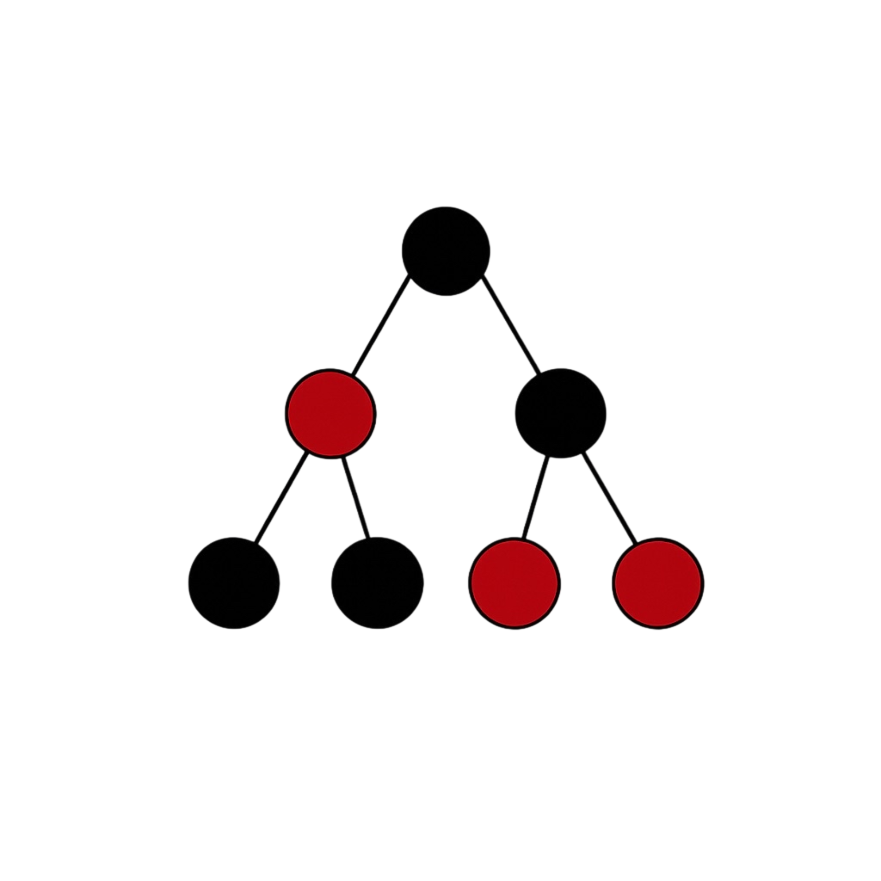
\includegraphics[width=0.38\paperwidth]{kcpc-logo.png}};
\end{tikzpicture}}
\titleformat{\section}{\large\bfseries\color{kcpc-red}}{}{0pt}{}
\setlist[itemize]{noitemsep,topsep=4pt}
\title{KCPC Week 3 Reading\\The Lambda Calculus: Functions, Computation, and Numbers}
\author{}\date{}
\begin{document}
\maketitle\thispagestyle{fancy}

Follow this guide alongside the slides and problem sheet. Start with the supplied Oxford notes, then use the accessible introductions for extra worked examples; the research bibliography in \emph{Week 3 Papers} gives the original sources. Page numbers below refer to the \emph{printed} pages of each text, rather than the PDF viewer counter.

\section*{I. The supplied further reading: Oxford lecture notes}
\subsection*{Lambda Calculus and Types (Andrew D. Ker)}
Oxford University Computing Laboratory, 16 lectures, Hilary Term 2009. Available locally at
\href{run:reading/lambdacalculus-lecture-notes-ht2009.pdf}{the supplied Oxford lecture-notes PDF} (in \texttt{reading/}).

\begin{itemize}
  \item \textbf{Chapter 1, \S\S1.2--1.5, pp.~2--7:} the grammar of terms, application association, free/bound variables, legal alpha-conversion and capture-avoiding substitution. Do this before Problems 1--5.
  \item \textbf{Chapter 4, \S4.1, pp.~43--44:} Boolean selectors, Church numerals, successor, zero test and predecessor. Compare with Problems 6--10. The chapter's introduction explains why numbers are encoded instead of built in.
  \item \textbf{Chapter 2, \S\S2.1--2.5, pp.~15--23 (after the workshop):} reduction sequences and the Church--Rosser theorem; why choosing different beta redexes need not change a normal form.
  \item \textbf{Chapter 3, \S3.1, pp.~31--33 (extension):} reduction strategies and why a concrete evaluator must choose which redex to contract.
\end{itemize}
The appendix on computational practice (pp.~109--115) gives answers to the notes' short calculation exercises; use it to check your attempts rather than to replace a proof.

\section*{II. Accessible introductions and worked examples}
\subsection*{Lecture Notes on the Lambda Calculus (Peter Selinger)}
Dalhousie University, revised 2013, arXiv:0804.3434. \url{https://arxiv.org/abs/0804.3434}
\begin{itemize}
  \item \textbf{\S2:} untyped terms, binding, substitution, alpha- and beta-conversion (Problems 1--5).
  \item \textbf{\S3:} Church encodings of Booleans, numerals and arithmetic (Problems 6--10).
  \item \textbf{\S4:} further theory of reduction; optional once the worksheet is complete.
\end{itemize}

\subsection*{Types and Programming Languages (Benjamin C. Pierce)}
MIT Press, 2002. Contents and chapter locations: \url{https://www.cis.upenn.edu/~bcpierce/tapl/contents.pdf}
\begin{itemize}
  \item \textbf{Chapter 5, \S5.1, pp.~51--58:} untyped lambda syntax, substitution and evaluation; clarifies exactly what a binder does.
  \item \textbf{Chapter 5, \S5.2, pp.~58--68:} currying, Booleans, pairs, Church numerals and recursion; alternate encoding examples.
  \item \textbf{Chapters 6--7, pp.~75--88 (optional):} nameless variables and an implementation of the calculus, particularly helpful if you want to build an evaluator after the two extended C++ homework tasks.
\end{itemize}

\subsection*{Church Numerals and Booleans (OpenDSA)}
Virginia Tech, Programming Languages, \S3.8. \url{https://opendsa-server.cs.vt.edu/ODSA/Books/PL/html/ChurchNumerals.html}
Interactive reduction traces for T/F, AND, successor, multiplication, predecessor and ISZERO. Use the animation to check a small input, then use iteration and induction to justify your answer for \emph{every} numeral.

\section*{III. Suggested order}
Read Ker \S\S1.2--1.5, solve Problems 1--5; read Ker \S4.1 and OpenDSA \S3.8, solve Problems 6--10; consult Pierce \S5.2 for pair encodings, then prove the stack invariants in Problems 11--12. For original research and precise bibliographic locations see \emph{Week 3 Papers}.

\end{document}
